% 03-simulation.tex

\chapter{Simulation}
\label{ch:sim}

Simulation is an important tool in hardware verification, together with formal verification \cite{YuanLu2001, Kumar1998}. It allows to ensure a design follows the expected behavior, as well as enabling comparison with the behavior of the manufactured circuit \cite{Ashenden1994}.

Furthermore, performing a correct simulation of our LLHD dialect allows us to assert that LLHD is fully representable in MLIR, as well as testing that new passes do not affect the semantics of the design. The latter in particular already showed to be valuable in Martin Erhart's work.

We propose a first prototype of a simulator using LLHD's MLIR representation, called \texttt{llhd-sim} (same as the LLHD reference simulator). For this prototype, we follow a similar approach to the \textit{LLHD-Blaze} simulator \cite{Schuiki2020}, by leveraging Just-In-Time (\textit{JIT}) code generation, in combination with an MLIR conversion pass from LLHD dialect to the LLVM dialect, to enable the execution of the units, and a sequential event-driven algorithm to carry out a behavioral simulation of the design. With this first research prototype, we can successfully simulate real-world designs such as a full \textit{Snitch} \cite{Zaruba2020} processor. A correctness and performance evaluation is provided in Chapter \ref{ch:eval}

%---------------------------------------------------------------------------------------------------

\section{Sequential Event-Driven Simulation}
Event-Driven Simulation algorithms \cite{Ashenden1994} view a physical design as a collection of physical processes. Physical processes then communicate with each other by reacting and generating time-stamped events, carrying the changes that happen to the physical signals during their execution. Each process can modify its local state but only communicate with other processes through events. This means that process execution during a time-step is independent of all other processes executed during that time-step, where a \textit{time-step} represents a unique instant in simulation time. The correctness of the simulation can thus be guaranteed if a process acts upon events in non-decreasing time-stamp order. We also note that no order is defined on independent events, and they can thus be processed in any order, without hurting the correctness of the algorithm. This holds in particular for events carrying the same timestamp, as those are always guaranteed to be independent.

\begin{listing}[ht]
    \caption{Sequential event-driven simulation algorithm.}
    \label{listing:seqEDS}
    \begin{minted}[
        frame=lines,
        framesep=2mm,
        baselinestretch=1.0,
        bgcolor=lightgray!10,
        fontsize=\footnotesize, linenos
        ]{c}
initialize all logical processes
while event-queue EQ not empty do
    set global simulation time to timestamp of first event in EQ
    pop the first element in EQ and resume destination process
    enqueue any new events scheduled by the process
    \end{minted}
\end{listing}

In a sequential implementation, as shown in Listing \ref{listing:seqEDS}, events are typically collected in an ordered queue of events (the \textit{event queue}). Here, events to be processed at later time-steps are stored in ascending time-stamp order. The body of the loop represents a simulation cycle, and in each cycle, one event is processed. Since the event-queue is ordered by the time-stamps, this also guarantees the correctness of the algorithm.

%---------------------------------------------------------------------------------------------------

\section{LLHD Simulation}
In LLHD, each unit (both entities and processes) represents one physical process. Each process can be sensible to a (sub-) set of all the signals present in the design.

In the case of an entity, its body is executed in its entirety each time one of the entity's owned signals (signals defined in that entity's body) or an input (or output) signal changes.

Processes on the other side can suspend their execution before the end of the body is reached. Furthermore, they can include control-flow loops and potentially run indefinitely. Generally speaking, the only way of completely stopping a process's execution is for it to reach a halt operation, which prevents the process from ever waking up again. A process execution thus usually resumes at the block targeted by the wait operation that suspended the process during its last execution, whenever the wait condition is met. The only exception to this is the first execution, where the process starts at the entry block.

\begin{listing}[ht]
    \begin{minted}[
        frame=lines,
        framesep=2mm,
        baselinestretch=1.0,
        bgcolor=lightgray!10,
        fontsize=\footnotesize, linenos
        ]{c}
initialize all logical processes
while event-queue EQ not empty do
    set global simulation time to timestamp of first event in EQ
    pop the first element in EQ
    apply the signal changes scheduled by the event
    wake up all sensitive units
    enqueue any new events scheduled by the units
    \end{minted}
    \caption{Revisited sequential event-driven simulation algorithm used to simulate LLHD.}
    \label{listing:seqLLHD}
\end{listing}

Listing \ref{listing:seqLLHD} revisits the sequential algorithm from Listing \ref{listing:seqEDS} to fit it to our needs. For each cycle, we build a \textit{wake-up queue}, which lists all the units that require to be executed in that cycle. After updating the global simulation time, the signal changes scheduled in the top-most event are first processed, filling the wake-up queue with the sensitive instances. All units in the wake-up queue are then executed (sequentially), and all the new events are finally queued in the event queue. We also note that we generate only one event for each unique instant, and this contains all the signal changes occurring in that instant, instead of having one event for each signal change. This allows us to both reduce the event-queue size and number of unit executions, while still guaranteeing simulation correctness due to the independence of such changes, as previously described. Also note that if the same signal is updated multiple times in the same time-step, only one change will be visible, obtained by applying all of them to the current value, in order of insertion in the event.


Following this revisited algorithm, we build a simulator using the structures described in Section \ref{sec:structs} to maintain the simulation state, and JIT compilation to enable the execution of LLHD units, as described in Section \ref{sec:execution}.

%-------------------------------------------------------------------------------

\subsection{Simulator Structures}
\label{sec:structs}
To be able to perform a simulation, we first need a means to keep track of the global simulation state and all the relevant information necessary to proceed through the simulation. To do this we use a series of data structures as basic building blocks of the global simulation state. In this section, we discuss their shape and use.

%---

\subsubsection{Time and Signals}
At the base of the simulator, we have a representation of time and signals.

A time unit can be simply represented by three values, representing real-time, delta step, and epsilon step. We also note that we have a fixed picosecond granularity in the simulator, and assume that the real-time values stored in the state have already been appropriately converted.

For signals, on the other hand, we require keeping track of some more information. Each signal can be uniquely identified through its name and owner instance. This enables us to identify signals in cases where their location in the global signal table is unknown. The name in particular is also required to identify the various signals in the generated simulation trace.

Each signal also owns a memory region in the heap, where its value is stored. A pointer to such a region is stored for each signal, together with its size (\ie, the number of bytes its type occupies in memory). We keep track of this information for making signals available to units during their execution (see Section \ref{sec:execution}), to process signal changes, and to generate a trace dump (see Section \ref{sec:trace}).

A signal update always results in a subset of all instances being triggered. To avoid needing to search each instance for each signal change, we store a list of all sensitive instances here as well.
% Figure \ref{fig:sig} shows the final shape of the signal structure.

% \begin{figure}[ht]
%     \centering
%     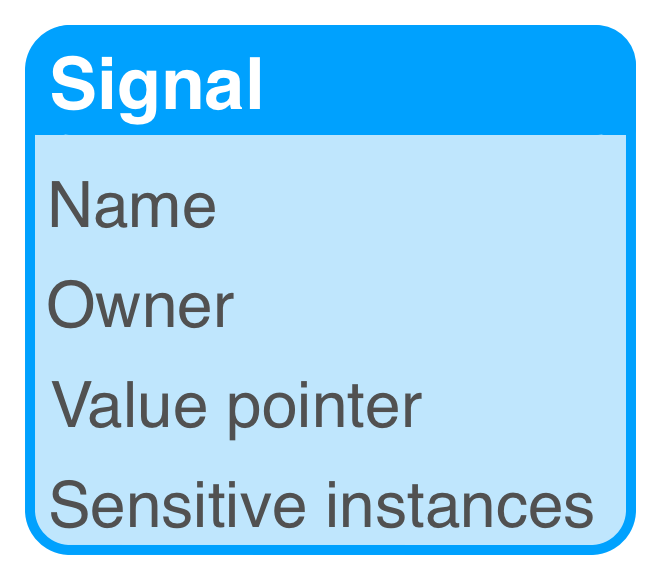
\includegraphics[width=0.4\textwidth]{gfx/Signal.png}
%     \caption{<PH> The data structure used to represent a signal in the global simulation state}
%     \label{fig:sig}
% \end{figure}

%---

\subsubsection{Instances}
Each instance represents a “copy“ of a unit, and different instances of the same unit can coexist, with different input and output signals connected to them. We thus keep track of various information about instances, starting from their name, the base unit they instantiate (to retrieve the unit function), as well as the instance's full hierarchical path, built during the state initialization (as discussed in Section \ref{sec:state}).

As mentioned, each instance has a set of signals it is sensible to. Those can be either owned by the instance itself, in case of an entity, or be connected through one of the input or output ports. For each of those signals, we store an entry in a local signal table, which contains the pointer to the signal value, a value representing it's offset in the first byte, and its index in the global signal table and instance signal table, to make them easily available to units during their execution. The use of this information will be explained in more detail later. Also note, that this does not correspond to the signal representation described above.

Entities and processes also require different local states during their execution. In the former case, the only additional local state-keeping required during execution is for the reg operation trigger values contained in the entity: to be able to detect a rising or falling edge of the trigger, the current SSA operand's value is not enough, but we always need information about its value in the previous execution of the instance.

For processes, on the other hand, more information is required: since processes can suspend their execution at any terminator in their body (through a wait operation), we need to keep track of where we need to resume execution. This can be achieved by indexing all the possible resume-points and storing the current index into the local state.

Another problem arises with value persistence, namely, since the body is no more fully executed, the process would resume and try accessing undefined values. We avoid that by storing all required values in the process' local state. A detailed description of how this is achieved can be found in Section \ref{sec:execution}. Finally, process suspension can also restrict the sensitivity of the instance to a given subset of its argument signals. This behavior can be represented by storing a flag for each signal in the instance's sensitivity list, indicating if sensitivity to a signal is currently enabled.

In some cases, a scheduled wakeup can be invalidated and should thus not be performed. This can happen on wait operations with both delay and signal arguments when one of the observed signals changes before the scheduled wakeup. We can achieve this behavior by keeping track of the timestamp at which we expect the process to wakeup. This way, when we process a scheduled wakeup, we can check if the current timestamp matches the one we expect and skip it if that is not the case. This way, invalidation of a scheduled wakeup can be achieved by setting the expected wakeup time to a timestamp in the past (\eg time-zero).

%---

\subsubsection{Events and the Event Queue}
An event (or \textit{time-slot}) in our simulator, as we defined at the beginning of this section, contains a list of signal changes rather than only one signal update. If multiple drives to the same signal are scheduled in the same time-step then the observable result will be a combination of all those changes, applied in order of insertion. We recall that this does not affect the correctness of the simulation, as the order of the updates scheduled for the same instant is not defined. Within a slot, we represent this by mapping signals to a list of signal updates, for each signal that has changes scheduled in that slot. Since processes can also have a timed suspension, we also keep a list of the processes scheduled to wake up in that slot.

With a slot as the base building block, we can construct the event-queue as a priority queue ordered by the slot's timestamp. Each slot thus becomes an entry in the queue and is placed in the correct position on insertion, such that popping the queue is always guaranteed to take the earliest possible event.

%---

\subsubsection{Global Simulation State and State Initialization}
\label{sec:state}
Finally, we can build the global simulation state. Here we store the current simulation time, as well as a global list of signals, the list of the instances present in the design, and finally the event queue.

To initialize the signal and instance structures, we analyze the input design during a first state initialization step, by recursively walking over its units for each inst operation, starting at the top-level (or \textit{root}) of the design. In this step, we gather the base information about instances and signals, such as their names and hierarchical paths, while the actual allocation of space for signal values and local states is performed in a later stage (see Section \ref{sec:execution}).

%-------------------------------------------------------------------------------

\subsection{Unit Execution}
\label{sec:execution}
Next, we need a means to emulate the behavior of a circuit. We observe that LLHD shares many similarities with the LLVM IR, and that a mapping from LLHD to LLVM IR is therefore mostly trivial. We can thus define an MLIR conversion pass from our LLHD dialect to the LLVM dialect, and then obtain the various units as callable function pointers, by feeding the converted module to a \textit{Just In Time} (\textit{JIT}) compiler (MLIR's \texttt{ExecutionEngine} in our case). As mentioned in Section \ref{section:mlir}, a conversion pass is mainly composed of a set of patterns that match a specific operation and define a legal conversion for it. Where we require direct interaction with the simulator's state, \eg, for spawning new events, we make use of a small runtime library, containing functions that can be called by the converted code.

In this section, we will describe how we can fully map LLHD to the LLVM dialect. We leave out a full description of some of the most trivial conversions, such as most of the bitwise operation, that can be mapped one-to-one to the LLVM dialect in our current implementation.

%---

\subsubsection{Mapping LLHD Types to LLVM Types}
\label{sec:typeconv}
For integers and tuples, we use MLIR's standard dialect types. The conversion for the integer is already defined by the standard-to-LLVM dialect conversion pass. For the tuple type, on the other side, no conversion is defined, and we are thus required to add a conversion from tuples to equivalent LLVM structs ourselves.

To map a signal to the LLVM dialect, we require keeping track of various important information, as previously mentioned. Furthermore, the result of an extraction operation on a signal is at all effect a new signal, but aliasing part of another signal instead of carrying some value. We will call such signals \textit{sub-signals}. These constructs are useful when only some parts of a signal require to be driven, for example, they enable driving only a single bit of an integer signal, or one element of an array.
Dealing with sub-signals requires us to make the following considerations:

\begin{itemize}
    \item We don't want to treat sub-signals as a special case: making this distinction would considerably increase the complexity of the conversion because, at the LLHD's IR level, there's no distinction between them. This would thus require some analysis to trace back the origin of the signal, as well as additional logic for all signal operations.
    \item Sub-signals are local values and do not live outside their unit's scope, as signals do. We thus don't want to store the sub-signals into the global state, as this would increase the complexity in the simulator engine too.
    \item Sub-signals can start at any element (or bit) of the original signal. This means that to fully represent sub-signals we would need bit-precision pointers. Memory, though, is generally byte-addressed, requiring us to use a representation able to mimic this behavior.
    \item Global signal information cannot be hard-coded into the unit mapping, as it’s generally not unique, but rather changes depending on which instance of the unit we want to run. We thus need a dynamic way to make each instance-specific signal table available to the lowered unit.
\end{itemize}

This requires all signals to have a representation that allows sub-signals to coexist along with global signals, to be local only, and to maintain all the required information to be able to perform drives. Using pointers allows us to hide this distinction from the generated code: local sub-signals can be represented by stack-allocated memory references, while global signals can live on the heap, hiding the distinction from other operations. A signal struct then contains all the information required to deal with both signals and sub-signals. This includes:

\begin{itemize}
    \item The pointer referencing the signal's value. In the case of sub-signals, this pointer is obtained by shifting the original signal's pointer to the byte where its value starts.
    \item The byte-offset. This enables representing the bit-granularity of sub-signal values. We also note that for normal signals, the offset will always be $0$, as their pointers are always generated by a \texttt{malloc} call. The bit-granularity behavior is thus only required because of sub-signals.
    \item The global signal index. This is necessary to retrieve the signal in the global state when driving. For sub-signals, this matches the original signal's index, so drives can be performed to the correct signal without any further processing.
    \item The instance signal index. This represents the index of the signal in the instance's local signal table and is used for filtering the signals a process is sensitive to at a given point in time.
\end{itemize}

As mentioned in Section \ref{section:llhdmlir}, LLVM arrays offer the flexibility we need for LLHD arrays, and we implemented our own type because we would have been limited to LLVM types, and to generally have an easier time working with that type. When mapping LLHD to LLVM dialect tough, we can now represent LLHD arrays as a one-to-one conversion to LLVM arrays of equivalent types, since we're mapping all LLHD types to LLVM types.

We currently map pointers one-to-one to LLVM dialect pointers. This means though, we currently have no way to represent an extract on an integer pointer, whenever the new pointer should be starting within a byte. In the future, we will need to maintain byte-offset information, similar to signals, for example by converting LLHD pointers to LLVM structs containing a pointer and a bit-offset. We note though, that this seems to be a relatively uncommon case, as it doesn't affect the simulation correctness in any of the examples in our test set.

Figure \ref{fig:types_mapping} recaps the mapping of LLHD types to LLVM dialect types.

\begin{figure}[ht]
    \centering
    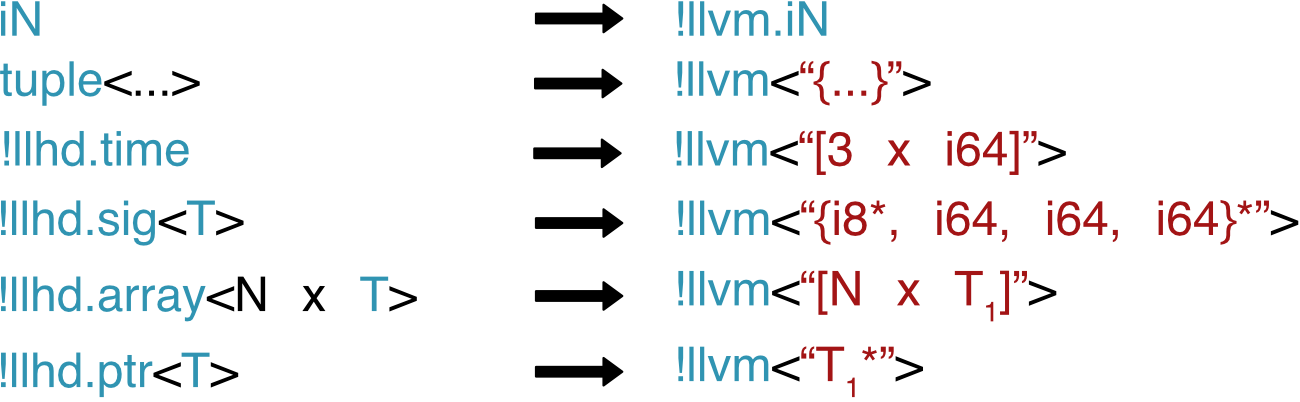
\includegraphics[width=\textwidth]{gfx/Types mappings.png}
    \caption[LLHD Types mappings to LLVM dialect types.]{LLHD Types mappings to LLVM dialect types. $T$ represents a legal LLHD sub-type, and $T_1$ represents its LLVM dialect equivalent.}
    \label{fig:types_mapping}
\end{figure}

%---

\subsubsection{Unit Conversion}
To represent entities and processes, we use LLVM functions with a static signature determined at compile-time, which replaces the original unit signature. The new signature contains a pointer to the global state and an array of signal structures representing the unit's signal table. A final argument represents the unit's local state. Here entities and processes will receive a pointer to the respective state type which is determined anew for each unit. More precisely, for entities, the local state will contain the value each reg operation's trigger assumed in its last execution. Processes on the other side require to maintain a local state for all the values that need to be persisted across process suspension, as well as a resume index, and a flags-array containing one entry for each argument signal, indicating if the process is currently sensible to the respective argument signal.

Since the original signature of the unit is stripped away, the signal operands are now undefined, and those signals reside instead as an element of the new signal table argument. For each of the signals in the signal table, we thus need to replace their uses with a pointer to the correct element in the signal table. We replace each signal operand with a \texttt{llvm.getelementptr} operation to the respective entry in the signal table. For argument signals, this operation is inserted at the beginning of the body, while for signals defined through the sig operation, it can be inserted at the operation's original location, as part of its conversion pattern.

To lower entity bodies, we observe that although they are defined to be following a data-flow paradigm, rather than control-flow (meaning the order the instructions appear in doesn't matter, and they should be executed following the \textit{Data-Flow Graph}, in short \textit{DFG}), LLHD still adheres to the SSA dominance condition (all SSA operands are declared before their use). This means that the order of execution dictated by the DFG will always be equivalent to the original order the instructions appear in. Also, at the time of implementing our dialect, there was no way to work around the dominance condition in MLIR, and \texttt{llhd.entity} bodies consequently have to adhere to it to be legal, further enforcing our observation. As a consequence, entity bodies' operations don't require to be re-ordered to follow the DFG, and we can inline them as they are into the converted entity function.

Process bodies require some further processing, namely, we need to generate logic for process suspension and resumption. Although process suspension is per se dictated by the \texttt{llhd.wait} operation, and this step seems thus more adequate to be part of the wait operation's pattern at first glance, we argue that the effects of this span across the whole process, making the latter's pattern a good place where to generate such logic. Furthermore, during the execution of the process lowering pattern, we have a broader view of the process easily available. In fact, a pattern of an MLIR pass usually receives only information about the operation it is matching, and tracking back information about other operations is not always trivial and sometimes requires arbitrary assumptions (\eg that another operation has not already been converted).

Enabling process suspension and resumption execution requires two main considerations:
\begin{enumerate}
    \item We require knowing where in the process' body the execution has to be resumed. We know that suspension can only happen at a block terminator, while resumption can only be at the beginning of a block. We can thus maintain an index, for each resume's target block, and insert a series of new blocks at the beginning of the body. Each of these blocks, we call them \textit{comparison-blocks}, compare the current index with one of the possible resume indexes, and then conditionally branches to the target block, in case the index matches, or to the next block otherwise. This mimics the behavior of the LLVM IR \textit{switch} instruction, which is, unfortunately, missing in the MLIR dialect. An example of this can be found in Figure \ref{fig:proclow}.
    \item We require to restore all the values, that the process uses after resumption, to the values they had before suspension. In a first naïve and very conservative implementation, we store each value that “escapes“ its defining block in the process' state, and load them from the local state whenever used outside their defining block. Since suspension can only happen at the end of a block, and resumption can only happen at the beginning of a block, this ensures we always have all the values we need available, at the cost of persisting additional values, which would otherwise not require to be persisted.  An example of this can be found in Figure \ref{fig:persistlow}. In the future, approaches such as Temporal Region Analysis could be used to determine which values actually require to be persisted and thus avoid redundant memory allocation and access. Another possibility worth exploring would be to use LLVM coroutines, of which we were unaware while implementing this.
\end{enumerate}

\begin{figure}
    \centering
    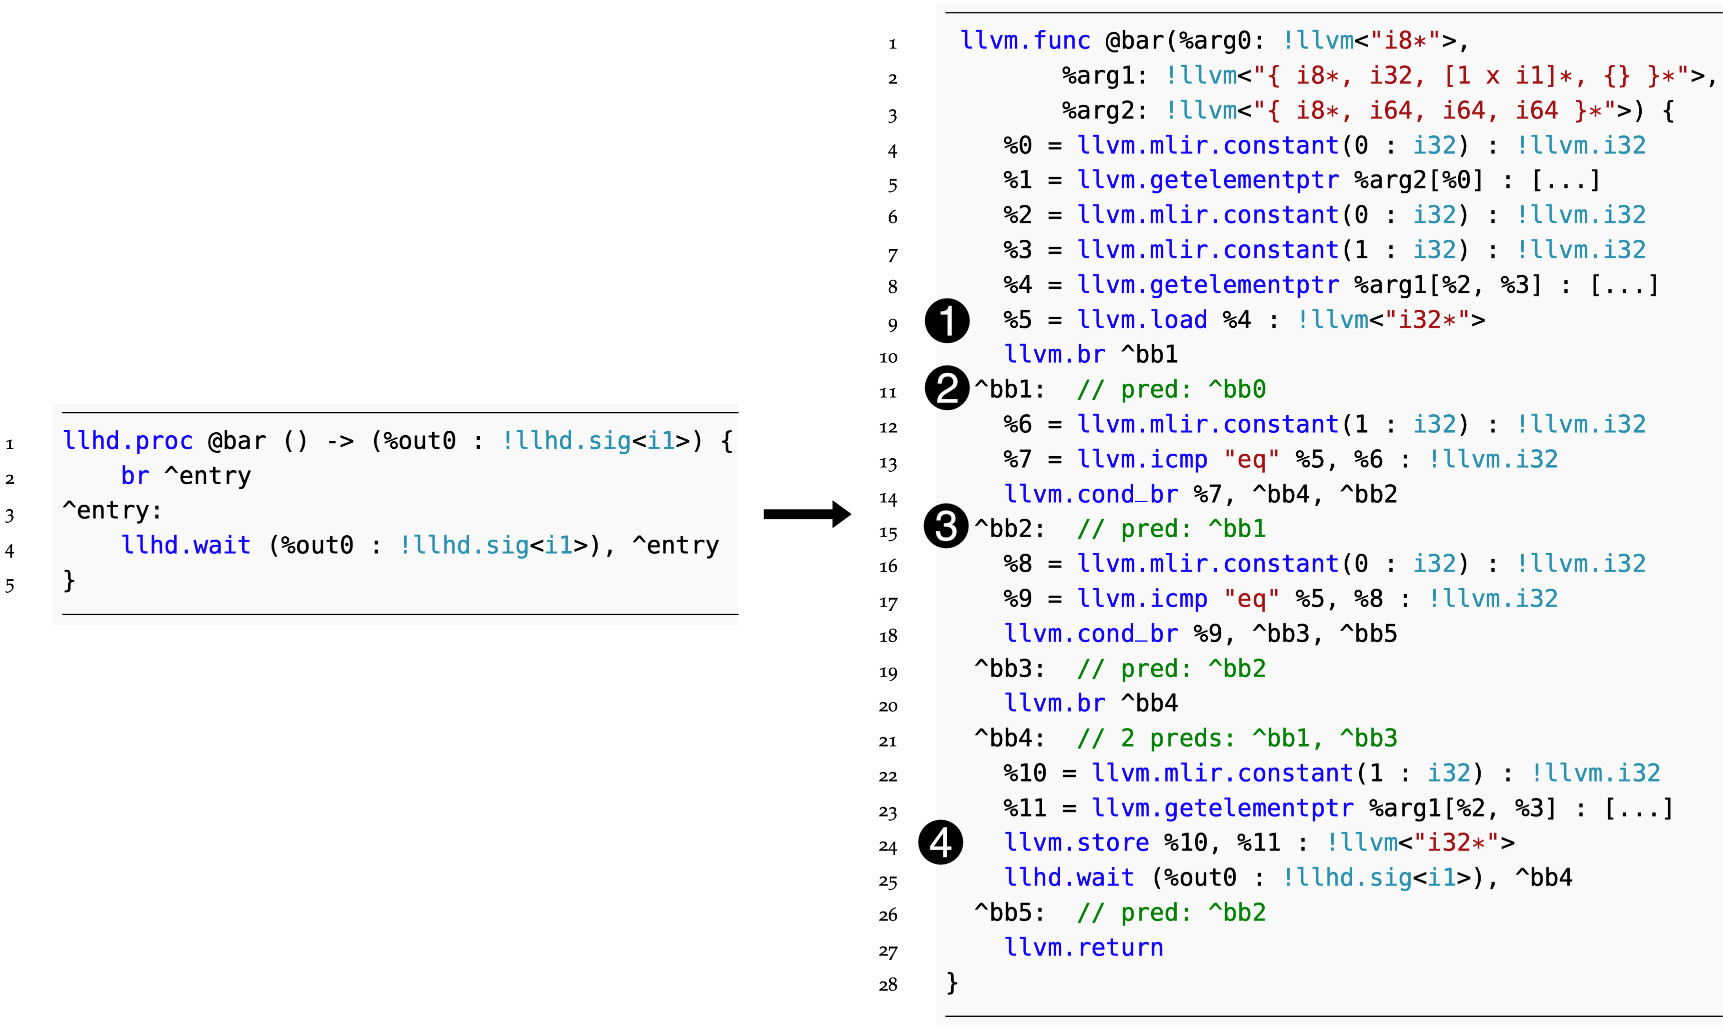
\includegraphics[width=\textwidth]{gfx/Resumelow.png}
    \caption[A simple example of process suspension logic generation.]{A simple example of process suspension logic generation. First, the resume index is loaded from the state (1). We then compare it against the first possible resume index (2). In case the index matches this value, the execution is resumed at \texttt{bb4}, else the index is compared against the second possible index (\ie, $0$) in the second comparison block (3). If that is the case, we are executing the process for the first time, and we jump to \texttt{bb3}. Otherwise, we are in an illegal state and interrupt execution by jumping to \texttt{bb5}. The resume index is finally updated before the wait operation (4). Non-relevant parts of code have been left out for the sake of readability (designated by [...]), as well as the \texttt{llhd.wait} operation conversion.}
    \label{fig:proclow}
\end{figure}

\begin{figure}
    \centering
    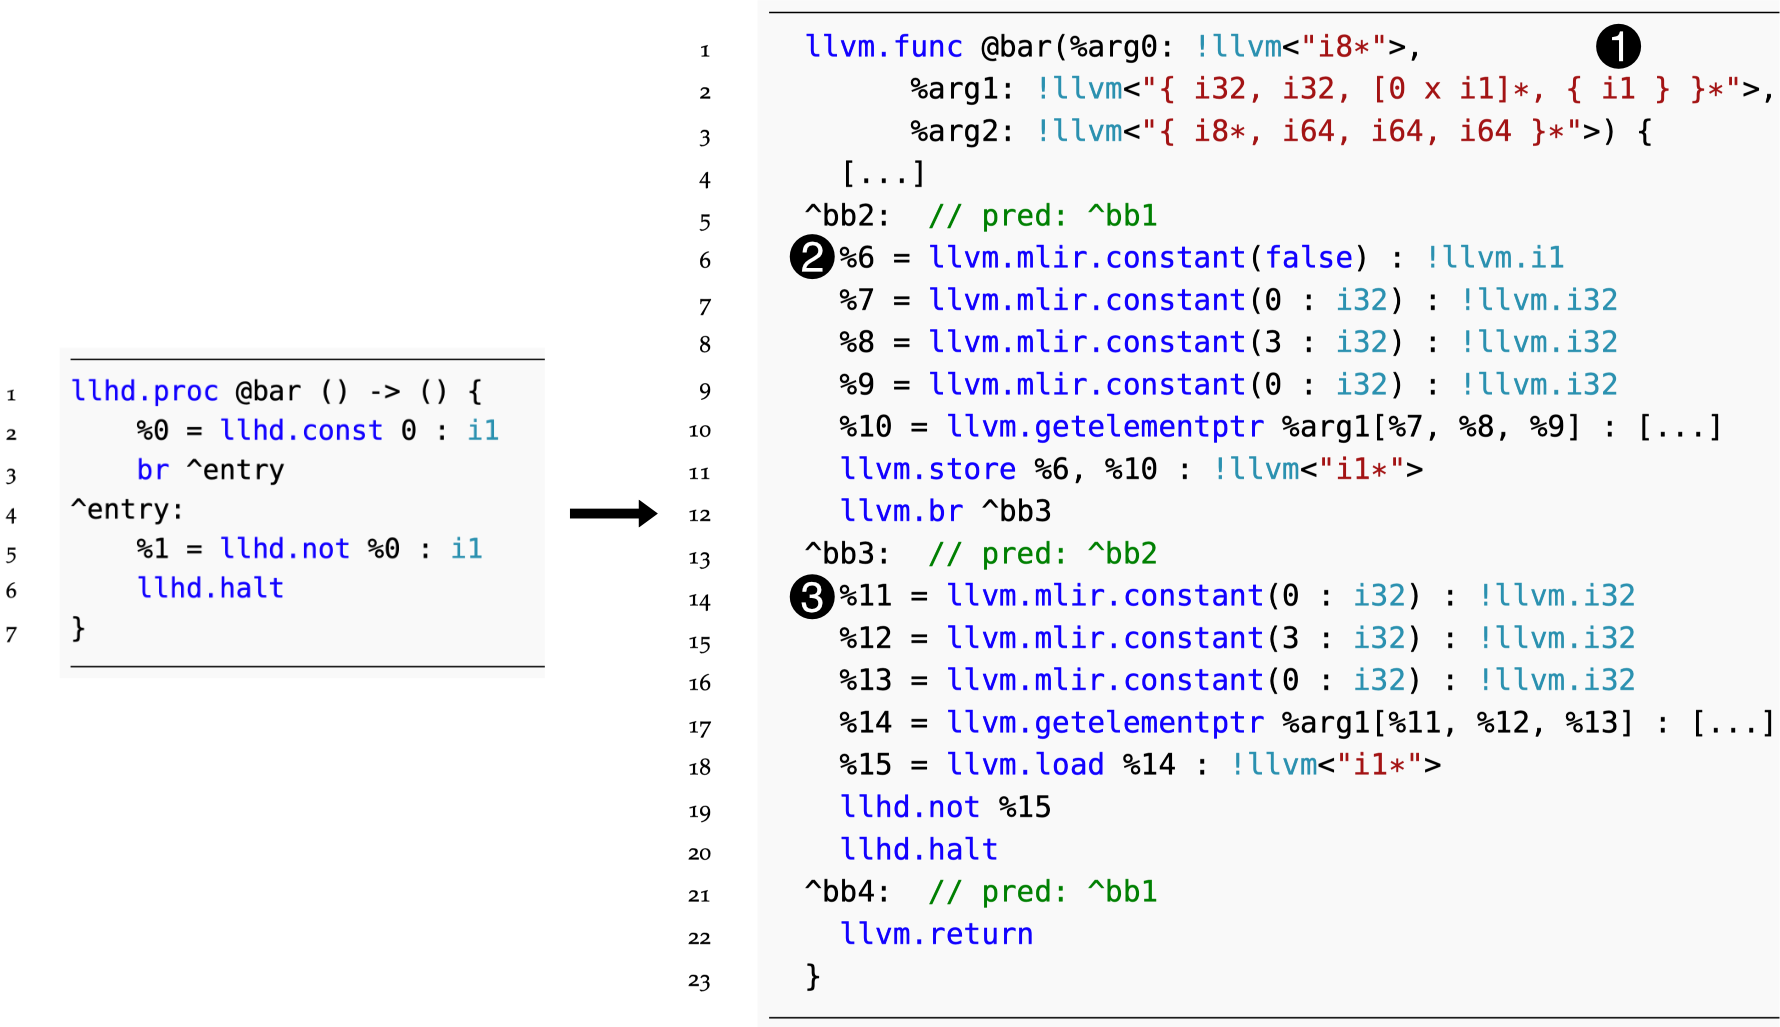
\includegraphics[width=\textwidth]{gfx/Persistlow.png}
    \caption[A simple example of value persistence logic generation.]{
        A simple example of value persistence logic generation. We can see that the boolean value appears in the process' local state (1). Since the boolean value escapes its defining block, it is stored into the local state (2) and subsequently loaded from it before it's use in the \texttt{entry} block (3). Non-relevant parts of code have been left out for the sake of readability (designated by [...]), as well as the conversion of the \texttt{llhd.not} and \texttt{llhd.halt} operations.
    }
    \label{fig:persistlow}
\end{figure}

Finally, since we're using the MLIR standard functions, we can directly use the standard dialect's conversion patterns to convert them to the LLVM dialect.

%---

\subsubsection{Instantiation Conversion}
As mentioned above, for each \texttt{llhd.inst} operation, a “copy“ of the unit is instantiated. This means that we require to also initialize a copy of each of the signals declared by the unit, as well as allocating memory for a new copy of the unit's local state. We accomplish this by generating an initialization function through the instantiation conversion.

In more detail, the \texttt{llhd.inst} conversion pattern walks over the target unit once,  generating \texttt{malloc} calls in the initialization function for each of the declared signals. We also note that we currently allocate double the required space for each of the signals. This is to cover the case of shifting signals, where probing a signal could result in accesses outside of the allocated memory region. Once support for the old LLHD shift instruction is removed, as discussed in Section \ref{section:llhdmlir}, we should also be able to reduce the space we allocate for signals.

Finally, we also generate \texttt{malloc} calls for the unit's local state and store all the generated pointers in the global state through some runtime function calls.

Important to note is that this approach requires us to guarantee that no other operation has been converted before the initialization function generation. Particularly, in the case of units, we lose information about the unit kind (whether it is an entity or a process) and signature. Similarly, for signals, we lose information about the carried type after the conversion. We thus convert the instantiation operations before anything else, by running a first partial conversion, only processing \texttt{llhd.inst} operations, followed by the full conversion. It is not yet clear if it would be worth separating this step in a new MLIR pass, as it would currently have no use outside this pipeline.

\subsubsection{Extraction conversion}
\label{sec:extrs}
The extraction operations are among the most complex LLHD operations. They can operate on almost any LLHD type, and the semantics of the LLVM dialect mapping varies slightly for almost all of those types. For integers and structured types, the conversion is straight forward: for integers, it is enough to shift the value and truncate it to the desired bit-width. For structured types, we can extract each required element and insert it in a newly defined value with the desired length. As explained in Section \ref{sec:typeconv}, for integer and signal pointers we require to change their view of the underlying value with a bit-granularity.

% Furthermore, the result of an extraction operation on a signal is at all effect a new signal, but aliasing part of another signal instead of carrying some value. We will call such signals \textit{sub-signals}. These constructs are useful when only some parts of a signal require to be driven, for example, they enable driving only a single bit of an integer signal, or one element of an array.

% Dealing with sub-signals requires us to make the following considerations:
% \begin{itemize}
%     \item We don't want to treat sub-signals as a special case: making this distinction would considerably increase the complexity of the conversion because, at the LLHD's IR level, there's no distinction between them. This would thus require some analysis to trace back the origin of the signal, as well as additional logic for all signal operations.
%     \item Sub-signals are local values and do not live outside their unit's scope, as signals do. We thus don't want to store the sub-signals into the global state, as this would increase the complexity in the simulator too.
% \end{itemize}

% This requires all signals to have a representation that allows sub-signals to coexist along with normal signals, to be local only, and to maintain all the required information to be able to perform drives.

% TODO: fix redundant explanation of signal representation => move to types mapping section!
% Local sub-signals can be represented by stack-allocated memory references, while global signals can live on the heap. A signal struct contains all the information required to deal with both signals and sub-signals. This includes:

% \begin{itemize}
%     \item The pointer referencing the signal's value. In the case of sub-signals, this pointer is obtained by shifting the original signal's pointer to the desired location.
%     \item The byte-offset. This enables the bit-granularity of pointers we described before. We also note that for normal signals, the offset will always be $0$, as their pointers are always generated by a \texttt{malloc} call, so the bit-granularity is only required because of sub-signals.
%     \item The global signal index. This is necessary to retrieve the signal in the global state when driving. For sub-signals, this matches the original signal's index, so drives can be performed to the correct signal without any further processing.
%     \item The instance signal index. This represents the index of the signal in the instance's local signal table and is used for filtering the signals a process is sensitive to at a given point in time.
% \end{itemize}

Extraction on signals, pointers, and arrays are also expected to be legal when accessing elements outside the bounds of the referenced memory region or value, in which case, the base value for the given type should be returned (\ie, $0$ for a 2-valued type such as a bit or \textit{X} for a SystemVerilog logic type). This behavior has currently only been implemented for arrays, by introducing additional boundary-checking logic. It is also partially mitigated by allocating additional space for storing signals, but no logic to test for the correct behavior is present in this case.

%---

\subsubsection{Insertion Conversion}
Insertions operations work on integer, tuple, and array types, inserting a slice (or element) into an existing value. The cases of array and tuple insertions can be trivially mapped to an LLVM insertion operations, or, in the case of slice insertion on arrays, one insertion per element.

For integer insertion, as shown in Figure \ref{fig:insert_int}, we can first mask the original value to set all the affected elements to $1$. Then we extend the slice to the target's width and shift it such that the slice is at the correct position. Finally, we need to apply a mask to the extended slice, such that it doesn't affect any bits outside the slice, before AND-ing it with the masked target.

\begin{figure}[ht]
    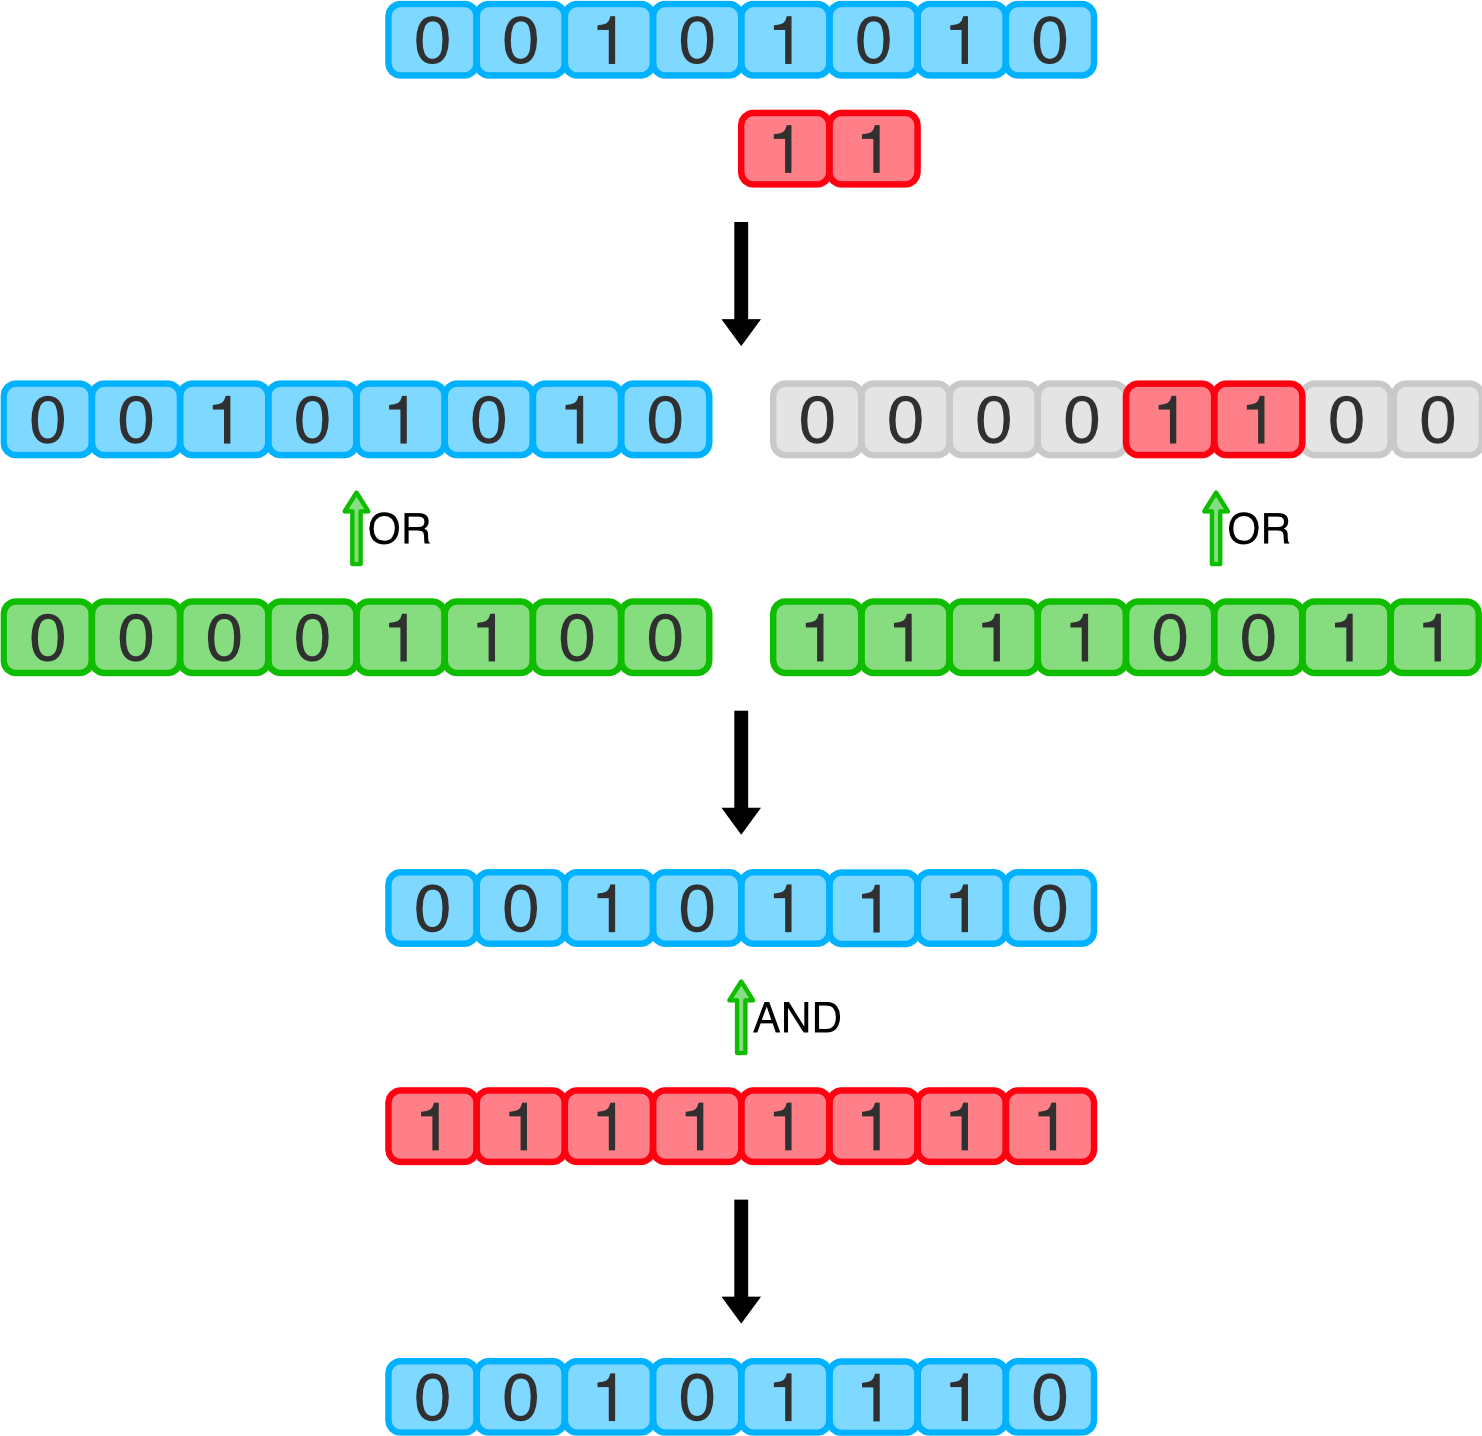
\includegraphics[width=\textwidth]{gfx/InsertInt.png}
    \caption[Illustration of the converted insertion semantics on integers.]{Illustration of the converted insertion semantics on integers. The blue areas represent the target value. The red values represents the slice we want to insert. The gray areas represent the values generated through sign extending and shifting the slice to adjust its position. Finally, the green values represent the masks generated to insert the slice.}
    \label{fig:insert_int}
\end{figure}
% TODO: add a figure!

%---

\subsubsection{Probing and Driving Signals}
Due to the potential byte-offset of sub-signal values, as previously described, we cannot probe a signal by just loading the value referenced by the signal pointer. Also, we can have a case where a sub-signal value spans only partially over the last byte of the memory region it is referencing, due to the variable bit-width of integers. This cannot happen to normal signals as they fully use the memory region they define (buffer region apart).

To probe an integer signal we thus always load the number of bytes required to represent the type in memory plus an additional byte to cover the case of sub-signals partially spanning across bytes. We then shift the loaded value by the given byte-offset, to ensure the loaded value starts at the correct position, and finally truncate the resulting value to the bit-width dictated by the signal's carried type. Figure \ref{fig:prb} shows an example of this process.

\begin{figure}[ht]
    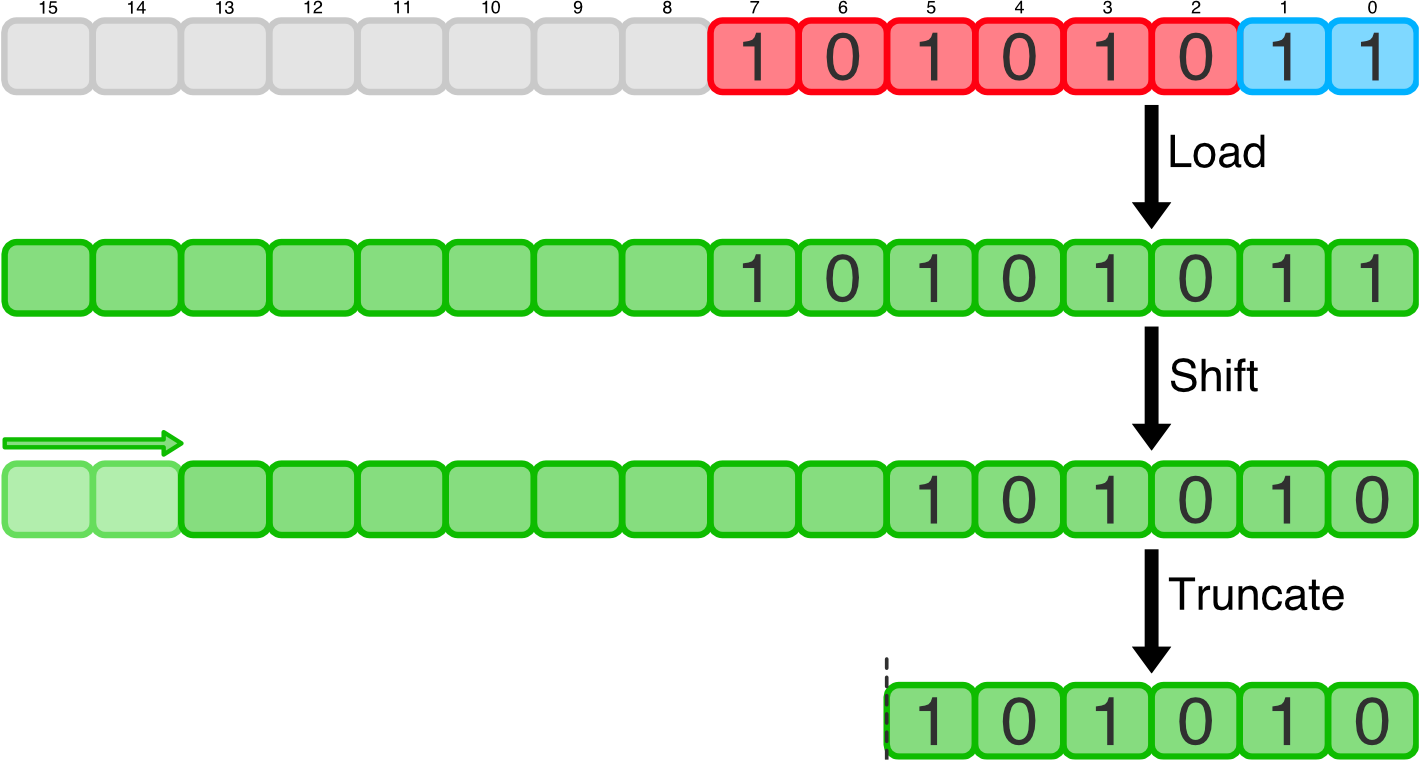
\includegraphics[width=\textwidth]{gfx/Probe.png}
    \caption[Illustration of the converted probe semantics.]{Illustration of the converted probe semantics. Here we want to probe an \texttt{i6} sub-signal (red area) of an \texttt{i8} signal (bits $0$
        through $7$). Finally, the gray area represents the extra buffer region allocated for the signal.}
    \label{fig:prb}
\end{figure}

Driving a signal requires us to spawn a new event in the event queue of the simulator, rather than directly update the stored signal value. As mentioned before, we interact with the state through a runtime library, and we do the same here. We use a runtime function, \texttt{drive\_signal}, to take the value to drive and add it as a change in the event queue, after the defined delay.

In the case a gating condition is present on the drive, we also generate additional blocks to conditionally execute or skip the drive based on the gating condition.

A reg operation conditionally drives one value out of a list of triggers and possible values. We can see this operation as a list of comparison blocks, similar to the ones we use for the process resumption logic, leading to a block containing a normal drive operation. The drive's arguments come from the newly generated block arguments, and each comparison block passes the elements of the respective reg-tuple to the target block through their conditional branch operations. This way, we can also reuse the drive operation conversion pattern and avoid some redundancy in the pass implementation.

%---

% \subsubsection{others?}


%-------------------------------------------------------------------------------

\subsection{Simulation Trace}
\label{sec:trace}
The simulation trace dump is the main output of a simulation. It lists all changes that occurred to the signals during the simulation. Traditionally, a simulator will work with a trace format similar to \textit{VCD}, the \textit{Variable Change Dump} format, which is also part of the SystemVerilog standard \cite{SV2018}. This format can then be used to visualize waveforms in programs such as \textit{GTKWave} \cite{gtkwave}, but has the downside of not being human-readable by itself, and automated comparison is not trivial (though utilities such as \textit{vcddiff} \cite{vcddiff} exist).

We propose a textual trace dump format, which is both human-readable without the aid of additional software, and easy to compare through widely available tools such as the \textit{diff} command-line tool.


In this textual representation, we use the following syntax:
\mint[showspaces, fontsize=\footnotesize]{c}|<timestamp>  <full-signal-hierarchical-path>  <value>|
\noindent The first element is the full timestamp, reporting the exact time, including delta and epsilon steps separated by one blank space. Next, we report a slash-separated (/) full hierarchical path of the updated signal. Finally, we print the new value in hexadecimal format, prefixed by \texttt{0x}, and $0$-padded to the nearest byte. The reason for this is mainly to keep a compact and coherent format throughout the whole trace. But this comes at the cost of not being able to distinguish, for example, an \texttt{i1} signal from an \texttt{i8} signal by purely looking at the trace.
For structured-type signals, we transpose the signal value dump by generating one trace entry for each element of the signal and appending the respective index to the hierarchical path.

A single signal generates one entry for each instance it is connected to, with the respective hierarchical path. Here we also note that our current implementation, we cannot retrieve the port names in the unit signatures, and we thus have to use the original name of the signal for all the hierarchical paths of the connected instances, rather than the port names.

A signal change also generates an entry in the trace only if the drive causes an actual change to the signal value. If a drive occurs, which does not change the signal value from its previous state, it generates no entry in the trace.

Within the same time-step, we define the order for the entries to follow the lexicographical order given by the full hierarchical paths. This allows a more normalized and well-formed comparison between the simulation traces.

Listing \ref{listing:toggle_trace} shows an example of trace for the first $10$ns of simulation of Listing \ref{listing:mlir_toggle}. Note that all the real-time values are listed in picoseconds. This is because we currently have assigned a static granularity of $1$ps for the simulator and don't perform any further formatting for the time values.

\begin{listing}[ht]
    \caption[An example of \texttt{llhd-sim}'s textual trace.]{An example of the trace generated by simulating the design in Listing \ref{listing:mlir_toggle} for the first $10$ns of execution.}
    \label{listing:toggle_trace}
    \inputminted[
        frame=lines,
        framesep=2mm,
        baselinestretch=1.0,
        bgcolor=lightgray!10,
        fontsize=\footnotesize, linenos
    ]{c}{examples/trace_toggle.txt}
\end{listing}

One of the main downsides of this textual representation of the signal dump is its size. When simulating full designs, this easily reaches multiple Gigabytes in size, which makes human inspection hard, as files of such size cannot be easily loaded in a text editor. Also, as the amount of signals in the design grows, the information gets too dense for effective human inspection.

For those reasons, we also propose some variations of this format, that can also be further explored in the future.

\begin{enumerate}
    \item Limit the traced signals to only the ones at the top level of the design. Those are usually the signals owned by the simulated test-bench and are often the ones of most interest for human inspection. The rationale for this is that the tested circuit can be seen as a “black-box“, and we can infer its correctness by the correctness of its results (the top-level signals).
    \item Merge all sub-steps into their real-time-step, such that only the final state of each signal is present for each real-time-step. This brings the trace closer to a typical VCD trace, where time sub-steps are not listed. Here we also group all signal changes that occur at the same time-step under only one timestamp, as shown in Listing \ref{listing:merged-syntax}. This allows identifying time-steps more easily when visually inspecting the trace.
    \item Trace only the top-level signals and merge the time sub-steps. This effectively merges the concepts introduced in variations 1. and 2., to further ease visual inspection.
    \item Filter out default-named helper signals. \texttt{moore} often introduces new helper signals during compilation to fully represent the original design. These will not have a name representative of the signal but are rather given an SSA ID as any other value in the IR. In non-LLHD simulators though, those signals are not represented, as they are not part of the original design. Filtering them out enables us to perform a comparison against well-established SystemVerilog simulators.
\end{enumerate}

\begin{listing}
    \caption{The syntax of the merged textual dump format.}
    \label{listing:merged-syntax}
    \centering
    \begin{minipage}{0.6\textwidth}
        \begin{minted}[fontsize=\footnotesize, showspaces]{c}
<timestamp>
  <full-signal-hierarchical-path>  <value>
  <full-signal-hierarchical-path>  <value>
  ...
            \end{minted}
    \end{minipage}
\end{listing}

We also provide a starting point for a modular tracing infrastructure, aimed at making it easier to add more dump formats in the future, such as VCD, which would enable a standard and well-established format.

